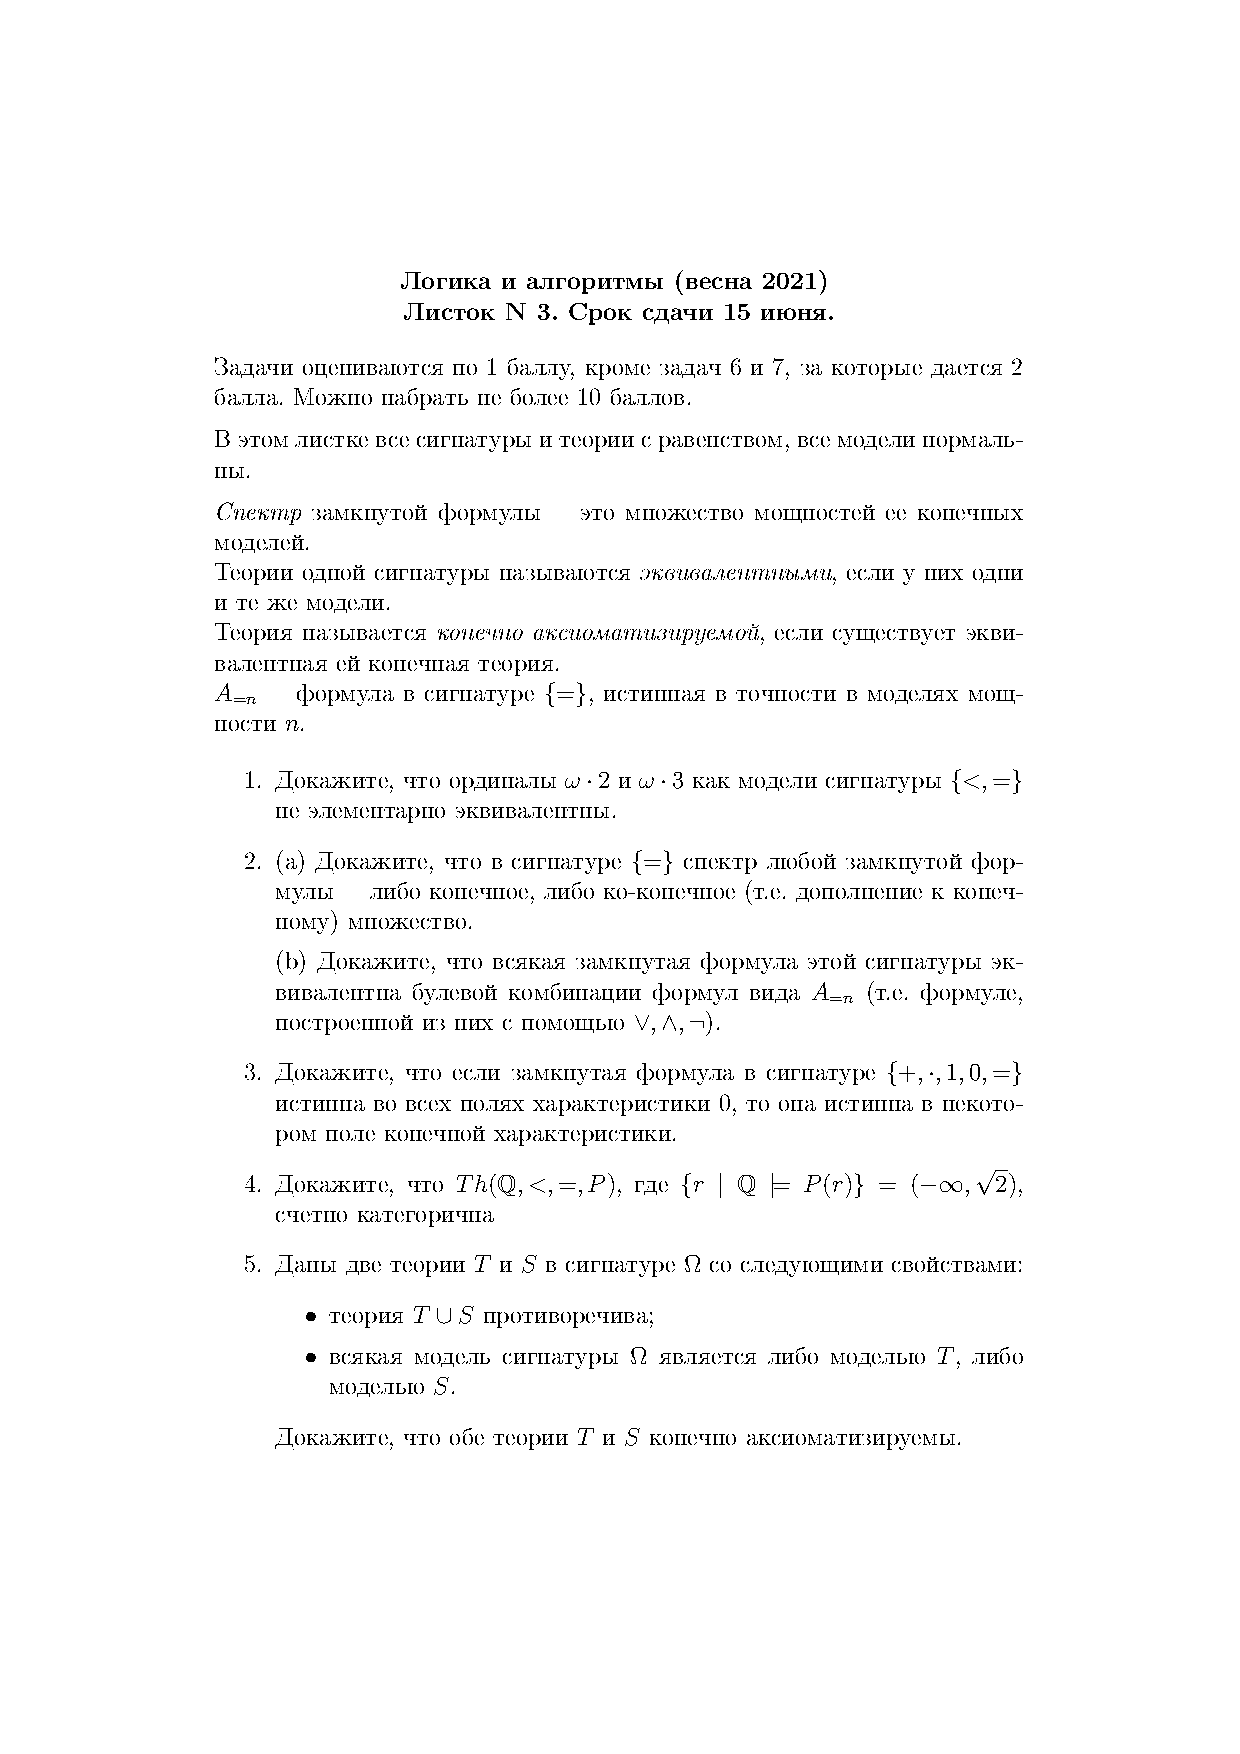
\includepdf[scale=1,pages=1-2]{Tasks/listok3}
\newpage
\section*{Решения}
\subsection*{Задача 1}
	Предъявим формулу, которая выполняется в одной модели, но не выполняется в другой:\\ Cуществует три различных элемента, у которых нет непосредственного предшественника. То есть $A = \exists x1, x2, x3\ (x1 != x2 \wedge x1 != x3 \wedge x2 != x3 \wedge \forall y\ (y < x_i \Rightarrow \exists z:\ y < z < x_i)$. $w*3 \models A,\ w*2 \models A$.
\vskip 0.4in

\subsection*{Задача 2}
\begin{enumerate}
\item[(a)] 
	Пусть $\operatorname{Sp}(A)$ -- спектр $A$. $\operatorname{Sp}(A)$ -- дополнение к $\operatorname{Sp}(\neg(A))$, так как если $A$ не истинна в $M$, то $\neg(A)$ истинна в $M$, а модели одинакового порядка, раз у нас сигнатура $\{=\}$, изоморфны. Тогда надо показать, что невозможно, что и $\operatorname{Sp}(A)$, и $\operatorname{Sp}(\neg(A))$ бесконечны. Пусть бесконечны, тогда у $A$ и $\neg(A)$ есть конечные модели сколь угодно большой мощности $\Rightarrow$ по теореме о подъеме есть и сколь угодно бесконечной. Возьмем тогда такие модели бесконечной мощности $k$. Получается, у $A$ и $\neg(A)$ есть модели одинаковой мощности одной сигнатуры. Как мы уже сказали, они должны быть изоморфны, то есть в них истинны одни и те же формулы, то есть в таких моделях мощности $k$ истинны и $A$, и $\neg(A)$, а так не может быть.
\item[(b)]
	Если $\operatorname{Sp}(A)$ конечен, то тогда у $A$ модели мощности $n_1, n_2, \ldots, n_k$. А еще модели одинаковой мощности изоморфны, то есть модели мощностей $n_1, \ldots, n_k$ будут моделями $A$. Значит, $A = \vee A_{= n}$ по $n = n_1, \ldots, n_k$.\\
	Если конечен, то $\operatorname{Sp}(\neg(A))$ конечное, тогда $\neg(A) \Leftrightarrow \vee A_{=n}$, тогда $A \Leftrightarrow \wedge\neg(A_{=n})$.
\end{enumerate}
\vskip 0.4in

\subsection*{Задача 3}
	Пусть $\{B\}$ аксиоматизирует теорию поля, $A$ замкнутая формула в сигнатуре, которая истинна в каждом поле характеристики $0$. Тогда $\{B\} \vee \{1 + \ldots + 1 \ne 0 \text{(n единиц)} | n \geqslant 1,\ n \in A\} \models A$ $\Rightarrow$ по теореме о компактности есть натуральное $m$, такое что $\{B\} \vee \{1 + \ldots + 1 \ne 0 \text{(n единиц)} | n = 1, \ldots, m\} \models A$ $\Rightarrow A$ истинна в каком-то поле $\operatorname{char} p > m$
\vskip 0.4in

\subsection*{Задача 5}
	$T \cup S$ противоречива $\Leftrightarrow$ есть формула $A$, такая что $T \cup S \vdash A$, $T \cup S \vdash \neg(A)$. Выводы конечные по определению, так что число использующихся аксиом конечно. Пусть из $T$ используются $\{t_1, \ldots, t_k\}$, из $S - \{s_1, \ldots, s_m\}$. В их объединении выводимы $A,\ \neg(A)$\\
	Теперь покажем, что $\{t_1, \ldots, t_k\} \sim T$. Покажем, что у них одинаковые модели. Если $M$ -- модель $T$, то $M$ -- модель $\{t_1, \ldots, t_k\} \subset T$. Наоборот от противного. То есть $M$ -- модель $\{t_1, \ldots, t_k\}$, но не модель $T$. По условию $M$ -- модель или $T$, или $S$. Значит, модель $S$. Тогда $M \models \{s_1, \ldots, s_m\} \subset S$. Раз $M \models \{t_1, \ldots, t_k\}$ по предположению, то $M \models \{s_1, \ldots, s_m\} \vee \{t_1, \ldots, t_k\}$. А в этом объединении выводимы $A$ и $\neg(A)$ (а значит, и истинны). Значит, $M \models A,\ \neg(A)$. Противоречие.\\
	Значит, $T \sim \{t_1, \ldots, t_k\} \Leftrightarrow T$ конечно аксиоматизируема. Аналогично $S$ конечно аксиоматизируема
\vskip 0.4in

\subsection*{Задача 7}
	Расширим сигнатуру, добавив в нее константу $c$. Добавим в $\operatorname{Th}(Q)$ схему аксиом $\forall n \exists x: x^n = c$.\\
	$\operatorname{Th}(Q) \vee \{\forall n \exists x: x^n = c\}$ выполнима по теореме о компактности (в каждой конечной подтеории есть лишь конечное число аксиом об извлечении корня. В качестве с возьмем достаточно большое рациональное число, из которого извлекаются все корни теории). По теореме о понижении мощности есть счетная элементарно эквивалентная ей модель $M$.\\
	Обедним сигнатуру до исходной. Чтобы показать, что $\operatorname{Th}(Q)$ не счетно категорична, предъявим две счетные неизоморфные модели. Покажем, что это $Q$ и $M$. От противного: пусть есть изоморфизм $\phi: M \sim Q$. Тогда $\phi(x) = \phi(0 + x) = \phi(0) + \phi(x) \Rightarrow \phi(0) = 0,\ \phi(x) = \phi(1 \cdot x) = \phi(1)\phi(x) \Rightarrow \phi(1) = 1$. Теперь посмотрим, как выглядит $\phi(c)$. Из $\phi(c)$ должен извлекаться корень любой степени. $\phi(c)$ рациональное, так что $\phi(c)$ или $0$, или $1$. Но $0$ и $1$ мы показали, что уже заняты. Так что изоморфизма нет.
\vskip 0.4in

\subsection*{Задача 9}
\begin{enumerate}
\item[(a)]
	$T$ не счетно категорично, т.е. не все счетные модели изоморфны. Явно покажем две счетные неизоморфные модели $T$. $M_1 = \{Z, S_1(x) = x + 1\}$, $M_2 = \{Z, S_2(x) = x + 2\}$. От противного: пусть они изоморфны, $\phi$ — изоморфизм. Тогда для любого $m$ из $M_1:\ \phi(m + 1) = \phi(m) + 2$. Тогда все $\phi(m)$ для всех $m$ из $M_1$ одинаковой четности. Но $\phi$ -- биекция. Противоречие
\end{enumerate}
